\section{Ejercicio 5}

$$
F(A,B,C,D) = \sum(3,7,11,13,14,15) \, , \, X = 6,2
$$

\subsection{Expresión mínima}

\begin{figure}[H]
    \centering
    \begin{karnaugh-map}[4][4][1][$D$][$C$][$B$][$A$]
        \minterms{3,7,11,13,14,15}
        \terms{6,2}{X}
        \implicant{3}{11}
        \implicant{7}{14}
        \implicant{13}{15}
    \end{karnaugh-map}
    \caption{Mapa de Karnaugh para la función}
\end{figure}

$$
F(A,B,C,D) = BC+CD+ABD
$$

\subsection{Simulación en Falstad}
\begin{figure}[H]
    \centering
    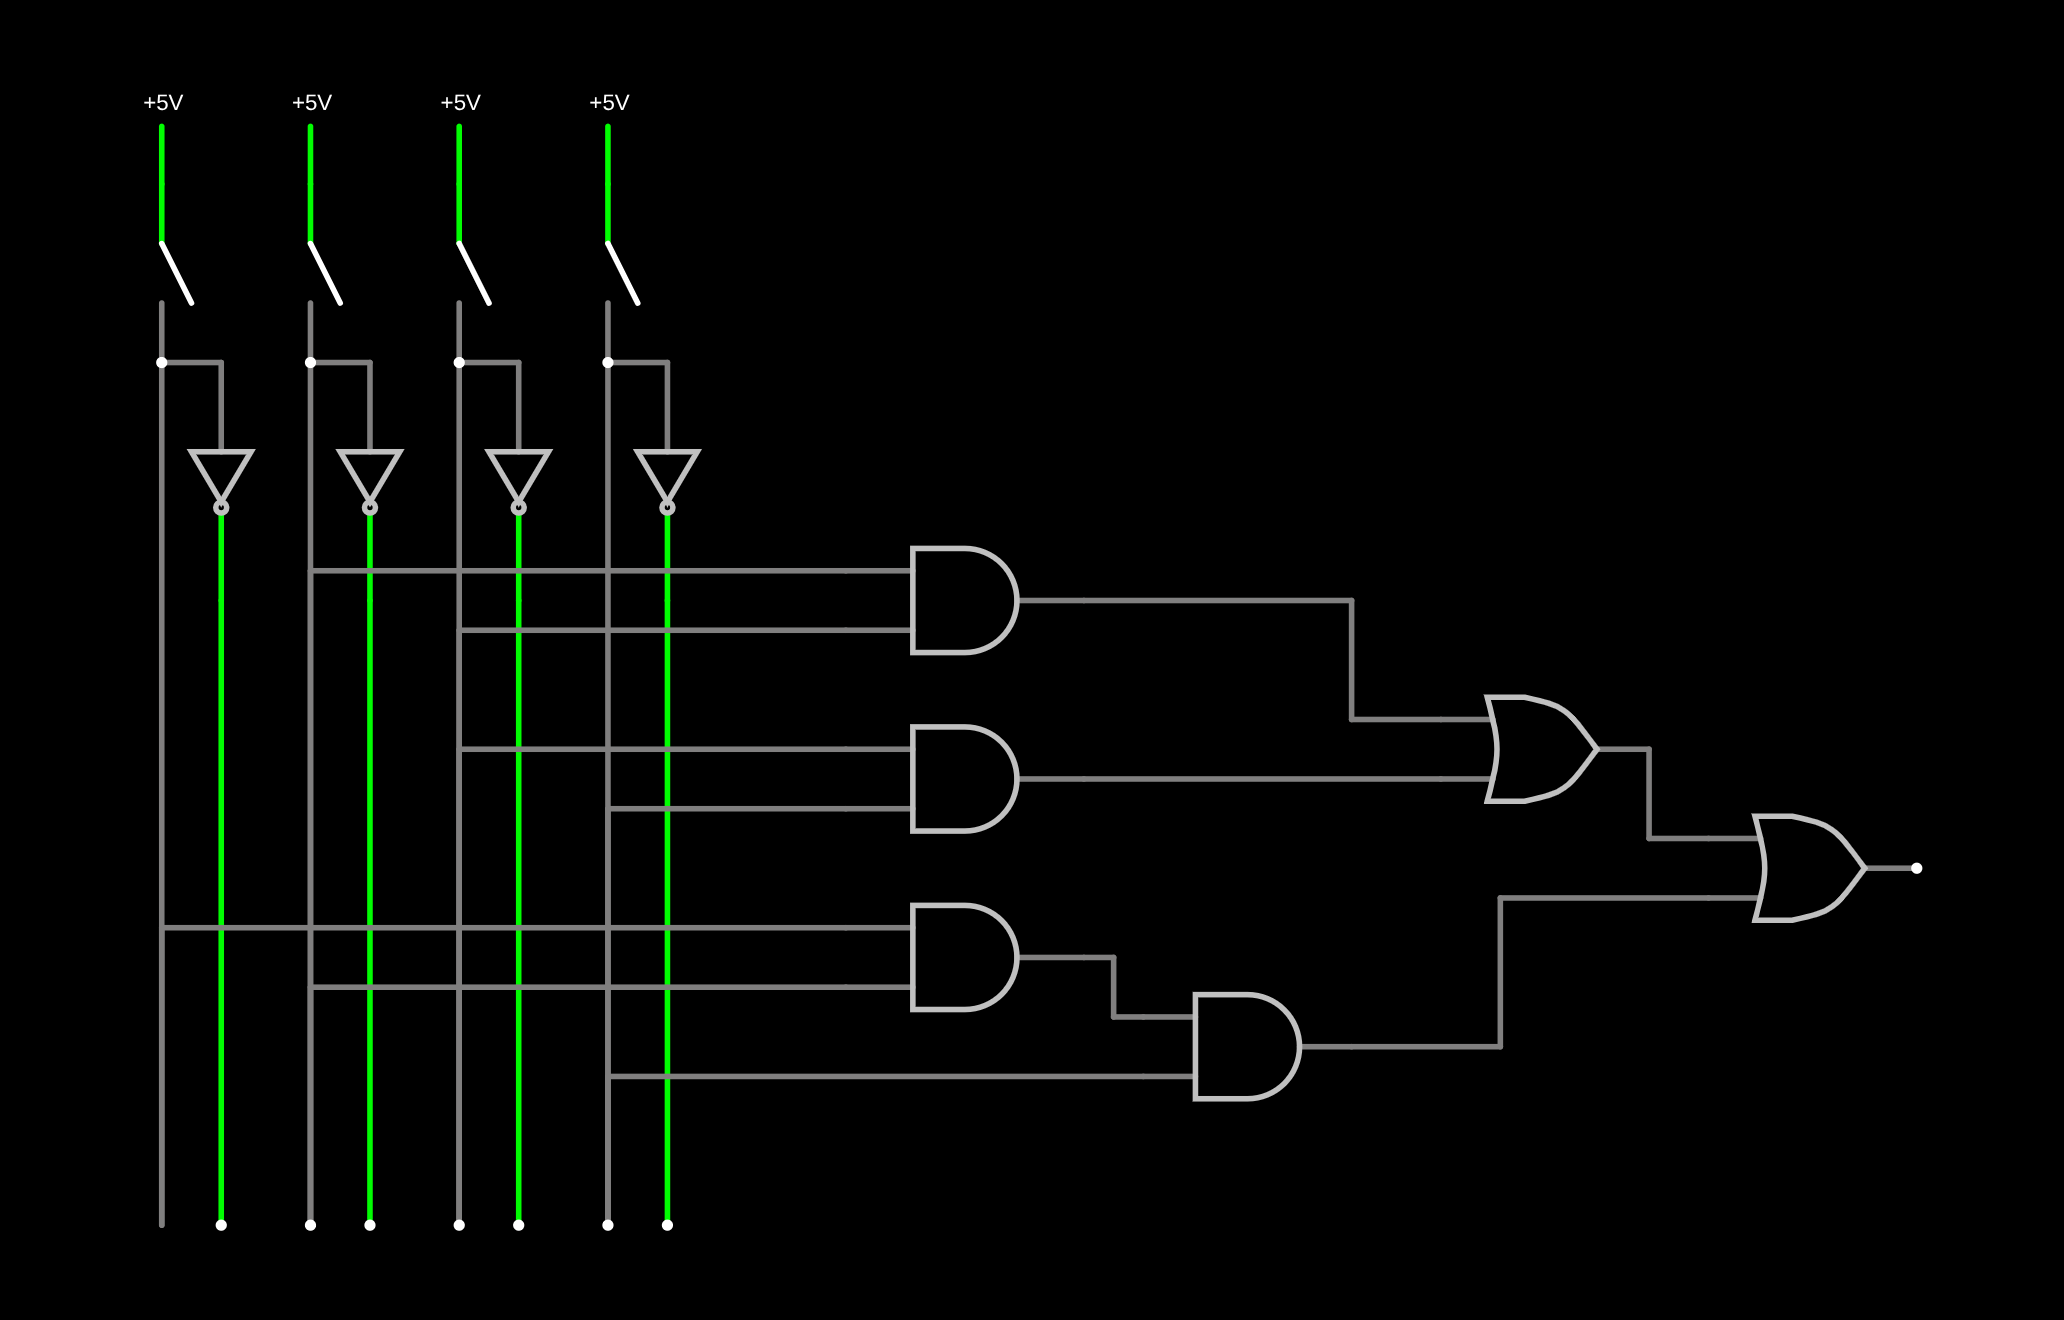
\includegraphics[width=0.6\textwidth]{img/Falstad/ej5.png}
    \caption{Simulación de la función en Falstad}
\end{figure}

\subsection{Descripción en Verilog}

\begin{Verbatim}[ frame=single, fontsize=\small, baselinestretch=1.2 ]
module ej5 (
    input A,
    input B,
    input C,
    input D,
    output F
);

assign F = B&C | C&D | A&B&D;

endmodule
\end{Verbatim}

\subsection{Captura del RTL}
\begin{figure}[H]
    \centering
    
\includegraphics[width=0.8\textwidth]{img/Xilinx/ej5.png}
    \caption{Captura del RTL en Xilinx}
\end{figure}